\documentclass[a4paper,11pt,titlepage]{article}
\usepackage{graphicx}
\author{Abrie Greeff\\B.Sc Hons (Computer Science)\\Department of Computer Science\\University of Stellenbosch}
\title{Statecharts}
\begin{document}
\maketitle
\tableofcontents

\section{Introduction}
Every person has a different level of understanding of each aspect of life. The problem is that this makes it difficult to explain a concept to someone that has less knowledge than the person that is explaining the concept. This problem becomes more evident in a professional environment where programmers and engineers have to explain how a product works to someone that is only interested in the final product.

A solution to this problem is to create a visualisation of the product. To further increase the easiness a product can be explained it may be necessary to add depth to the visualisation. This means creating a visualisation that has different levels of understanding. Each level will therefore increase the amount of information about a certain aspect of the product. The bottom most level will therefore contain the most information about the product and the top level the least.

D. Harel~\cite{Harel} proposed such a model for visualising information called statecharts. Statecharts is an extension of deterministic finite automata (DFAs) as defined in~\cite{sipser}. DFAs have rules to move between states called transition functions. These transition functions are also contained in statecharts. The difference between these two are that in a DFA the whole system can be seen but in a statechart occlusion occurs. This is because statecharts have different levels as defined above.
Fig.~\ref{Figure:statechart} shows a typical statechart and Fig.~\ref{Figure:dfa} shows an equivalent DFA. There is one more difference between DFAs and statecharts and that is that DFAs have accept states and statecharts does not. This is because statecharts are mostly used to model real-time systems performing under certain input and DFAs to model decisions made on certain input. Under most circumstances statecharts will execute to infinity and only stop if an event occurred that the system was not designed to handle. Because of this when a statechart is executing at a certain level and receives an unknown event that not one of the possible DFAs it is executing can handle the system will go back a level and check if that level is able to process the event. This process continues until a level is reached that is able to handle the event. If the statechart was unable to process the event the statechart will stop functioning. This report will focus on implementing statecharts and defining an input syntax used for creating statecharts.



\begin{figure}[htbp]
   \centering
   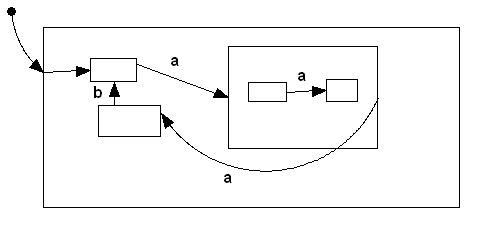
\includegraphics[width=7cm]{state.png}
   \caption{A statechart}
   \label{Figure:statechart}
\end{figure}

\begin{figure}[htbp]
   \centering
   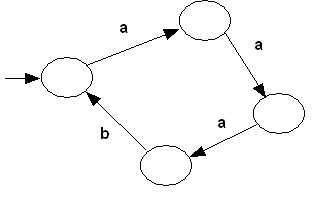
\includegraphics[width=7cm]{dfa.png}
   \caption{An equivalent DFA}
   \label{Figure:dfa}
\end{figure}
\newpage
\section {Input Syntax}
The input syntax I developed is loosely based upon Grail input that is commonly used to define input syntax for DFAs. I first needed to decide how the different levels of a statechart could be added to this syntax. Because this is only an input syntax it is not necessary to worry how a application will use the syntax. The final syntax has four rules and one optional rule. The order in which these rules are parsed are however important in creating the correct statechart.
\subsection{Rule 1}
\begin{verbatim}
ROOT <level>
\end{verbatim}
The first rule is only needed once in the input file. This defines what level the statechart enters at when it starts traversing the statechart.

\subsection{Rule 2}
\begin{verbatim}
NODE <level>
\end{verbatim}
Each level of the statechart has a certain amount of DFAs executing in parallel. Before these DFAs can be defined this rule is needed to define what level of the statechart we are defining DFAs in. Every DFA definition that follows will be allocated to this level until a new level is defined.

\subsection{Rule 3}
\begin{verbatim}
START <state>
\end{verbatim}
This rule defines a start state for a DFA. This start state will be defined at the same level of the node (see Rule 2) that is currently active. Every start state that is defined at this level will run in parallel with each other when this level is entered.

\subsection{Rule 4}
\begin{verbatim}
<state> <input> <transition state> 
\end{verbatim}
The transition rule for every state is defined by this rule. These states will also be saved on the same level as the current node (see Rule 2). The states can however be one of two possibilities, another state at the same level, or a node above or below it.

\subsection{Rule 5}
\begin{verbatim}
<state> FINAL
\end{verbatim}
This rule is an optional rule and is only provided for compatibility with DFAs. This defines if a state is able to accept and return to the state that called it.

\subsection{Example}
\begin{verbatim}
ROOT 0
NODE 0
START 0.0
0.0 a 0.1
0.1 a 0.2
0.2 b 0.0
START 0.3
0.3 a 0.4
0.4 b 0.5
0.5 a 0.3
NODE 0.1
START 0.1.0
0.1.0 b 0.1.1
NODE 0.4
START 0.4.1
0.4.1 c 0.4.2
0.4.2 d 0.4.1
\end{verbatim}
This input file would define a statechart as in Fig.~\ref{Figure:example}

\begin{figure}[htbp]
   \centering
   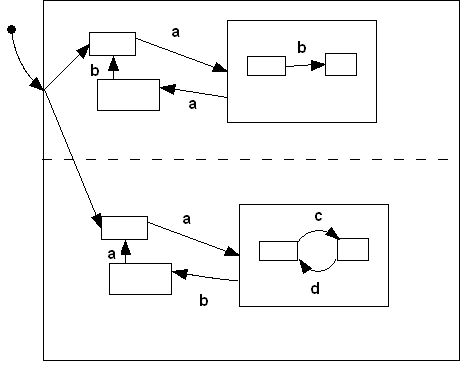
\includegraphics[width=7cm]{example.png}
   \caption{Corresponding statechart}
   \label{Figure:example}
\end{figure}

\section{Implementation}
The application for traversing statecharts was developed in Java 1.5.0~\cite{Java}. The first step was to load an input syntax file and load all the text into an \emph{ArrayList} object. This object was chosen because the list would be cleared starting from the first item and thus all operations on the object would be \emph{O(1)}.

An object class \emph{state} was created to store all data for a certain level. All the \emph{state} classes were stored in a hash table and indexed with their name as the key. The hash table was chosen because the time to search for an object is very fast and the key will always be known. The \emph{state} class stored information about all the start states on its level, the accept states, all the transitions that occur on its level and a link to the hash table that contain all the other \emph{state} classes.

When all this data was loaded, the main program started to read the input file to traverse the statechart. Before we can describe how the system operates it is necessary to note how a level is loaded before being traversed. When the system sees it needs to move to a certain level it finds all the information about that level by loading the corresponding \emph{state} information from the hash table into a new thread class \emph{child}. The thread \emph{child} will then know everything that is needed about that level as well as the parent that called it. If the thread is the initial level then it will not have a parent. By using threads the system will be able to run multiple concurrent operations.

The system starts by loading the root thread. When a new character is read from the input file it will be passed to this thread. The root thread will then do one of two possible operations on all the DFAs it is currently running. If it has a child thread running in one of its DFAs the character will then be passed down to that child until it reaches a level that doesn't have a child. If one of the DFAs is currently in a state that is not running a child it will check if it has a transition function defined for that character and transition to that state. These operations happen on all threads on the lowest level. If a state receives a character that does not satisfy a transition function that state will reject and stop the thread. If all DFAs on its level have stopped the level will destroy itself and notify its parent that it could not handle the event. The parent will then  check if itself can handle the event. If it can, the transitions will continue on its level. Otherwise that level will notify its parent and so forth. These events will continue until all the characters are read and the program will then exit.
\newpage
\section{Testing}
Testing was conducted with four statecharts. The first was a simple modification of a DFA into a statechart as in Fig.~\ref{Figure:test1}.
The second was the same statechart modified a bit to have two parallel running DFAs as in Fig.~\ref{Figure:test2}.
The third test was the second modified to jump between a low level and a top level as in Fig.~\ref{Figure:test3}.
The last test was the same as the second test but ten levels was now added to the statechart to see if it was possible to have so many levels. These tests showed me that my initial configuration of the application where all the threads instead of the level information was stored in the hash table proved to be incorrect.

\begin{figure}[htbp]
   \centering
   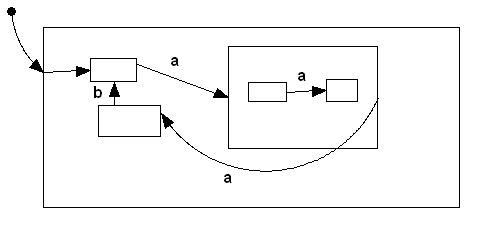
\includegraphics[width=7cm]{state.png}
   \caption{Test 1}
   \label{Figure:test1}
\end{figure}

\begin{figure}[htbp]
   \centering
   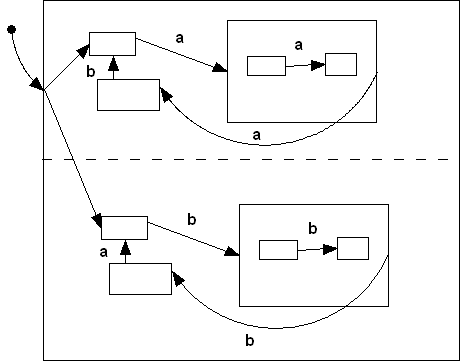
\includegraphics[width=7cm]{test2.png}
   \caption{Test 2}
   \label{Figure:test2}
\end{figure}

\begin{figure}[htbp]
   \centering
   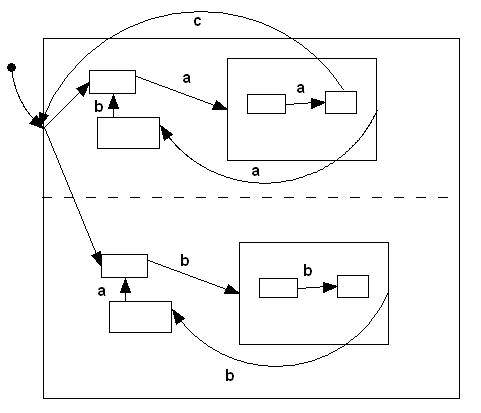
\includegraphics[width=7cm]{test3.png}
   \caption{Test 3}
   \label{Figure:test3}
\end{figure}
\newpage
\section{Summary}
This implementation proved to be very interesting. The threads proved to be a bit more daunting than initially expected but once they were sorted out proved to be very useful. The input syntax I developed proved to be very simple and efficient and loading it into my application was very easy. Although the application did not cover all the possible situations that a statechart could handle it was satisfactory. The only improvement that could definitely could be made is to add a visual interface to show how the statechart looked and was traversed.


\begin{thebibliography}{9}
\bibitem{Harel} D Harel,
\emph{On Visual Formalisms}, 
Communications of the ACM, Vol. 31 Nr. 5, 1988, pp 514-530

\bibitem{Java} 3D Studio Max,
\emph{Autodesk 3ds Max},	
[Online], Available from \emph{http://www.autodesk.com/3dsmax }

\bibitem{sipser} M Sipser,
\emph{Introduction to the Theory of Computation},
1997, p. 35


\end{thebibliography}
\end{document}
